\documentclass[a4paper, 14pt]{article}
\usepackage[utf8]{inputenc}
\usepackage[russian]{babel}
\usepackage{graphicx}

\usepackage{listings}
\lstset{
	language=C++,
	numbers=left,
	frame=single,
	breaklines=true,
	breakatwhitespace=true,
	title=lstname,
	tabsize=4	
}

\usepackage{color}
\usepackage{amsmath}
\usepackage{pgfplots}
\usepackage{url}

\usepackage{titlesec}
\titleformat*{\section}{\LARGE\bfseries}
\titleformat*{\subsection}{\Large\bfseries}
\titleformat*{\subsubsection}{\large\bfseries}
\titleformat*{\paragraph}{\large\bfseries}
\titleformat*{\subparagraph}{\large\bfseries}

\begin{document}
	\begin{titlepage}
		\begin{center}
			\begin{LARGE}
				Отчет по лабораторной работе №2\\
				по курсу "Анализ алгоритмов"\\
				по теме "Изучение алгоритмов умножения матриц "
			\end{LARGE}
			
			\begin{Large}
				\vspace{10cm}
				Студент: Барсуков Н.М. ИУ7-56\\
				Преподаватель: Волкова Л.Л.,
				Строганов Ю.В.
			\end{Large}
		\end{center}
	\end{titlepage}
	
	\tableofcontents
	
	\newpage
	\section*{Введение}
	
	Умножение матриц — это один из базовых алгоритмов, который широко применяется в различных численных методах, и в частности в алгоритмах машинного обучения. Многие реализации прямого и обратного распространения сигнала в сверточных слоях нейронной сети базируются на этой операции. Так порой до 90-95\% всего времени, затрачиваемого на машинное обучение, приходится именно на эту операцию. Так же это один из немногих алгоритмов, который позволяет эффективно задействовать все вычислительные ресурсы современных процессоров и графических ускорителей. Поэтому не удивительно, что многие алгоритмы стараются свести к матричному умножению — дополнительная расходы, связанные с подготовкой данных, как правило с лихвой окупаются общим ускорением алгоритмов

	\newpage
	\section{Аналитическая раздел}
	
	\newpage
	\subsection{Постановка задачи}
	
	Цель: изучить алгоритмы умножения матриц
	
	Для достижения поставленной цели требуется решить следующие задачи:
	
	\begin{enumerate}
		\item Изучить
		\begin{enumerate}
			\item Классический алгоритм умножения
			\item Алгоритм Винограда
		\end{enumerate}
		\item Реализовать указанные выше алгоритмы
		\item Разработать и реализовать оптимизированный алгоритм Винограда
		\item Выбрать модель оценки трудоемкости
		\item Сделать замеры алгоритмов
		\item Сравнить теоритические и экперементальные оценки трудоемкости 
		\item Сделать вывод
	\end{enumerate}
	
	В данный момент существуют несколько алгоритмов перемножения матриц. Ниже в таблице 1 приведен их список с коэффициентом ω, который показывает сложность алгоритмов $O(n^\omega)$
		
	В данном разделе будет приведено математическое описание алгоритмов перемножения матриц. Буду рассмотрены 3 подхода: классический, алгоритм Винограда и оптимизированный алгоритм Винограда.
	
	\subsection{Классический подход}
	
	Предположим, что необходимо получить матрицу $C_{(a,c)} = A_{(a,b)} * B_{(b,c)}$. Для нахождения значений элементов матрицы $C_{(a,c)}$ используют следующие выражение
	
	\begin{center}
		\begin{math}
		C_{i,j} = \sum_{K}(A_{i, k}B_{i,k})
		\end{math}
	\end{center}
		
	Классический алгоритм напрямую реализует эту формулу

	\subsection{Алгоритм Винограда}
	
	Можно заметить, что элементы из суммы выражения 1 можно переписать как:
	
	\begin{math}
		A_{i, k-1}B_{k-1,j} + A_{i,k}B_{k,j} = (A_{i,k-1} + B_{k,j})(A_{i,k} + B_{k-1,j}) - A_{i,k-1}A_{i,k} - B_{k-1}B_{k,j}
	\end{math}
	
	т. е. как сумму произведения сумм и двух произведений. Учитывая, что упомянутые два произведения можно рассчитать заранее для обработки двух элементов матрицы теперь нужно не сложение и два умножения, а умножение и два сложения, что проще с точки зрения вычислений. Таким образом, алгоритм Винограда состоит в следующем.
	
	\begin{enumerate}
		\item Совершить расчет заранее двух произведений для каждого ряда и столбца матрицы-результата (одно произведение считается для ряда, другое для столбца). Для хранения результатов используется промежуточный буфер
		\item По вышеприведённой формуле осуществить расчёт каждого элемента матрицы;
		\item В случае, если в произведении $A_{(a,b) X B_{b,c}}$ b – нечётное число, пройтись во второй раз по матрице, дополняя элементы $C_{i,j}$ недостающим элементом (который не был описан вышеописанной суммой). Можно заметить, что пункт 3 необходимо выполнять только в некоторых случаях, но если это происходит, то получается существенное увеличение времени работы алгоритма.
	\end{enumerate} 
	
	\subsection{Оптимизированный алгоритм Винограда}
	
	\begin{enumerate}
		\item Внутри тройного цикла накапливать результат в буфер, а вне цикла сбрасывать его в ячейку матрицы.
		\item Заменить MulH[i] = MulH[i] + … на MulH[i] += … (аналогично для MulV),
		где MulH и MulB – временные массивы для предварительного рассчета сумм произведений
		
	\end{enumerate}
	
	\newpage
	\section{Конструкторский раздел}
	
	\subsection{Алгоритмы}
	
	\subsubsection{Классический}
	
	\vspace{1cm}
	
	\begin{figure}[]
		\centering
		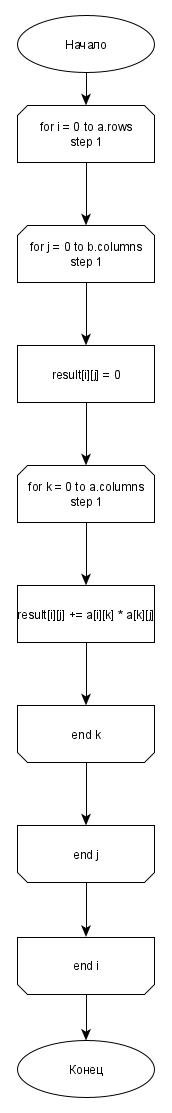
\includegraphics[height=20cm]{Схемы/simple}
		\caption{Классический алгоритм}
		\label{fig:simple}
	\end{figure}
	
	\subsubsection{Алгоритм Винограда}
	
	\vspace{1cm}
	
	\begin{figure}[]
		\centering
		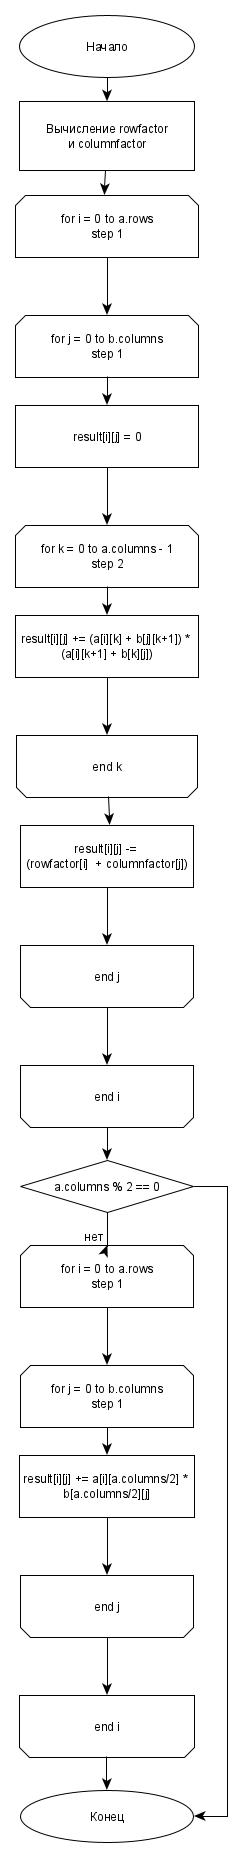
\includegraphics[height=20cm]{Схемы/vinograd}
		\caption{Алгоритм Винограда}
		\label{fig:vinograd}
	\end{figure}
	
	
	\subsubsection{Алгоритм Винограда улучшенный}
	
	\vspace{1cm}
	
	\begin{figure}[]
		\centering
		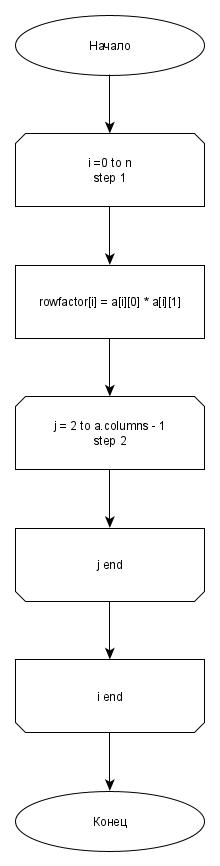
\includegraphics[height=20cm]{Схемы/rowfactor}
		\caption{Rowfactor}
		\label{fig:rowfactor}
	\end{figure}
	
	
	\newpage
	\section{Технологический раздел}
	
	\subsection{Требования}
	
	Данный программный продукт должен умножать 2 матрицы
	
	
	\subsection{Выбор языка и среды разработки}
	
	Для решения данной поставленной задачи, мной был выбран язык с++ по причине быстродействия, по скольку в нашем случаи пользователю необоходимо как можно быстрее получить результат выполенния нашего алгоритма.
	
	Так же мной используются среда разработки под названием VS Visual Studio по причине удобства и функциональности. И так же желания изучить данную среду по лучше.
	
	\subsection{Интерфейс}
	
	Интерфейс представляет из себя простую консоль в котором пользователь взаимодействует с помощью изменения параметров программы
	
	\subsection{Листинг}
	
	\subsubsection{Классический}
		
	\lstinputlisting[firstline=58, lastline=79] {../Matrix.cpp}
	
	\subsubsection{Винограда}
	
	\lstinputlisting[firstline=105, lastline=156]{../Matrix.cpp}
	
	\subsubsection{Виногорада улучшенный}
	
	\lstinputlisting[firstline=159, lastline=215]{../Matrix.cpp}
		
	\newpage
	\section{Исследовательский раздел}
	
	\subsubsection{Debug}
	
	\begin{tabular}{|c|c|c|c|c|}
		\hline 
		Размерность\ Алгоритм & Классик & Классик ул. & Винограда & Винограда ул. \\ 
		\hline 
		100 & 140 & 78 & 78 & 62 \\ 
		\hline 
		200 & 982 & 422 & 452 & 312 \\ 
		\hline 
		300 & 3775 & 2949 & 3615 & 3026 \\ 
		\hline 
		400 & 6645 & 3145 & 3768 & 2839 \\ 
		\hline 
		500 & 21575 & 6240 & 7410 & 5648 \\ 
		\hline 
		600 & 26782 & 10811 & 12823 & 9865 \\ 
		\hline 
		700 & 35584 & 19036 & 21590 & 16645 \\ 
		\hline 
		800 & 53805 & 34741 & 39250 & 32885 \\ 
		\hline 
		900 & 94474 & 68406 & 82135 & 66846 \\ 
		\hline 
		100 & 141414 & 105394 & 111638 & 131493 \\ 
		\hline 
	\end{tabular} 

	\begin{tikzpicture}
		\begin{axis}[
			title = Сравнение, 
			xlabel=Размер матрицы,
			ylabel=Количество тиков]% coordinates
	
		\addplot[color=blue] coordinates { (100, 140)
									(200, 982)
									(300, 3775)
									(400, 6645)
									(500, 21575)
									(600, 26782)
									(700, 35584)
									(800, 53805)
									(900, 94474)
									(1000, 141414) };
		
		\addplot[color=black] coordinates{ (100, 78)
									(200, 422)
									(300, 2949)
									(400, 3145)
									(500, 6240)
									(600, 10811)
									(700, 19036)
									(800, 34741)
									(900, 68406)
									(1000, 105394) };
								
		\addplot[color=red] coordinates { (100, 78)
									(200, 452)
									(300, 3615)
									(400, 3768)
									(500, 7410)
									(600, 12823)
									(700, 21590)
									(800, 39250)
									(900, 82135)
									(1000, 105394) };
		
		\addplot[color=red] coordinates { (100, 62)
									(200, 312)
									(300, 3026)
									(400, 2839)
									(500, 5648)
									(600, 9865)
									(700, 16645)
									(800, 32885)
									(900, 66846)
									(1000, 131493) };
		
	\end{axis}
	\end{tikzpicture}
	
	\subsubsection{Release}
	
	\begin{tabular}{|c|c|c|c|c|}
		\hline 
		Размерность\ Алгоритм & Классик & Классик ул. & Винограда & Винограда ул. \\ 
		\hline 
		100 & 31 & 31 & 31 & 31 \\ 
		\hline 
		200 & 219 & 125 & 249 & 219 \\ 
		\hline 
		300 & 733 & 438 & 702 & 421 \\ 
		\hline 
		400 & 2544 & 1138 & 1373 & 845 \\ 
		\hline 
		500 & 3822 & 1826 & 2826 & 1966 \\ 
		\hline 
		600 & 9549 & 3562 & 5109 & 3764 \\ 
		\hline 
		700 & 25319 & 20239 & 25877 & 16430 \\ 
		\hline 
		800 & 33092 & 29881 & 31061 & 30251 \\ 
		\hline 
		900 & 132864 & 76041 & 56852 & 70562 \\ 
		\hline 
		1000 & 208147 & 235230 & 114093 & 128083 \\ 
		\hline 
	\end{tabular} 
	
	\begin{tikzpicture}
	\begin{axis}[
	title = Сравнение, 
	xlabel=Размер матрицы,
	ylabel=Количество тиков]% coordinates
	
	\addplot[color=blue] coordinates { (100, 31)
		(200, 219)
		(300, 733)
		(400, 2544)
		(500, 3822)
		(600, 9549)
		(700, 25319)
		(800, 33092)
		(900, 132864)
		(1000, 208147) };
	
	\addplot[color=black] coordinates{ (100, 31)
		(200, 125)
		(300, 438)
		(400, 1138)
		(500, 1826)
		(600, 3562)
		(700, 20239)
		(800, 29881)
		(900, 76041)
		(1000, 235230) };
	
	\addplot[color=red] coordinates { (100, 31)
		(200, 249)
		(300, 702)
		(400, 1373)
		(500, 2826)
		(600, 5109)
		(700, 25877)
		(800, 31061)
		(900, 56852)
		(1000, 114093) };
	
	\addplot[color=red] coordinates { (100, 31)
		(200, 219)
		(300, 421)
		(400, 845)
		(500, 1966)
		(600, 3764)
		(700, 16430)
		(800, 30251)
		(900, 70562)
		(1000, 128083) };
	
	\end{axis}
	\end{tikzpicture}
	
	
	\newpage
	\section{Вывод}
	
	Можно заметить значительно преимущество алгоритма Винограда над классическим алгоритмом, которое растет пропорционально размерности матриц. Улучшения для алгоритма Винограда дают чуть лучший результат, чем оригинальный алгоритм, но не всегда.
	Намного большую эффективность дает добавление флага оптимизации компилятора 03.
	
	
	\newpage
	\section{Заключение}
	
	В ходе работы были исследованы два алгоритма умножения матриц: классический и Винограда. На квадратных матрицах размера от 100 до 1000, заполненных произвольными числами, было проведено сравнение скорости этих алгоритмов между собой, а также с их оптимизированными программными методами вариантами. Исследования проводились при компиляции с оптимизациями и без. Установлено, что алгоритм Винограда на достаточно больших размерах матриц (больше 800) дает значительный прирост в производительности. Программные оптимизации дают хороший результат при отключенных оптимизациях компилятора и незначительно лучший, а иногда и худший результат при включенных.
	
\end{document}

